\documentclass{beamer}
% use this instead for 16:9 aspect ratio:
%\documentclass[aspectratio=169]{beamer}
\usepackage{etex}
\usepackage{verbatim}
\usepackage{multimedia}
\reserveinserts{28}
\usetheme{ETHbeamer}

\colorlet{ETHcolor1}{ETHc}
\colorlet{ETHcolor2}{ETHc}

\author{Benjamin Ellenberger}
\institute{INI:  Institute of Neuroinformatics}

\title{Multiple chaotic central pattern generators with learning for legged locomotion and malfunction compensation}

\date{2016-01-27}

%%TODO: Optimize with presentation tips

% uncomment if you do not want to use a department logo
%\deplogofalse

\usepackage{color}
\usepackage{listings}
\usepackage{caption}
\usepackage{todonotes}

\DeclareCaptionLabelFormat{algocaption}{Algorithm} % defines a new caption label as Algorithm x.y

\lstnewenvironment{algorithm}[1][] %defines the algorithm listing environment
{   
    \lstset{ %this is the stype
        numbers=left, 
        numberstyle=\tiny,
        basicstyle=\tiny, 
        keywordstyle=\color{black}\bfseries\em,
        keywords={, initialize, if, then, else, foreach, do, while, begin, end, repeat, until, run, } %add the keywords you want, or load a language as Rubens explains in his comment above.
        numbers=left,
        xleftmargin=.04\textwidth,
        #1 % this is to add specific settings to an usage of this environment (for instnce, the caption and referable label)
    }
}
{}

\begin{document}

\titleframe

\section{}

\section{Introduction to the basic mechanism}

\begin{comment}
-Many researchers have proved that CPG-based control is an effective method for locomotion control of bio-inspired walking robots.

-A chaotic system can be controlled into showing periodic dynamics, so as to be implemented as a CPG to accomplish the locomotion control of a bio-inspired hexapod robot.
-So far, the chaotic CPG system contains only one oscillator, which has difficulties dealing with leg malfunction.
-We extend the single chaotic CPG system to multiple coupled CPG systems. Therefore each leg can perform identical patterns for normal walking or independent patterns to cope with malfunction.



-In the end, we show the real robot experiments to verify the performance of our methods.

Methods
-The single chaotic CPG is extended to multiple CPGs, specifically to six for a hexapod robot and to four for a quadruped robot.
-We choose a master CPG arbitrarily which dominates the pattern when synchronized, while the other CPGs are clients which can oscillate independently when desynchronized.
-When some legs are malfunctioning, they lose synchronization and can show different patterns such that the robot can maintain its forward walking in a straight line.
-An annealing-based learning algorithm is applied to automatically find the best matching oscillation frequencies to compensate for the malfunction.

Results
-The proposed algorithm was evaluated first in a physics simulation of a quadruped as well as a hexapod robot.
-It was also tested on the real hexapod robot AMOSII with three scenarios where one, two and three legs were disabled.
-In these three experiments, the robot deviated from its original trajectories and failed to pass the tunnel when the remaining legs with identical periods.
-The robot can walk in a straight line and successfully pass the tunnel when the learned combination of leg periods was employed.

Conclusions
-We demonstrate that multiple coupled chaotic CPGs with learning can be used for legged locomotion and malfunction compensation.
-When all legs are functional, the CPG units stay synchronized to show identical movement; if some legs are malfunctioning, the CPGs can desynchronize and learn a proper combination of leg periods to compensate for the malfunctioning legs.
\end{comment}

\begin{frame}
\begin{figure}
\center
\includegraphics[width=1\textwidth]{figs/abstract-a.pdf}
\end{figure}
\footnote{From [1]}
\end{frame}

\begin{frame}

\frametitle{Problem}
\begin{figure}
\center
\movie[autostart,showcontrols]{\includegraphics[width=0.6\textwidth]{figs/AMOS_3.jpg}}{figs/videos/nphys1508-s3.mpg}
\end{figure}
\footnote{From [2]}
\end{frame}

\begin{frame}
\frametitle{Meet AMOS II}
\begin{figure}
\center
\includegraphics[width=0.9\textwidth]{figs/AMOSII-cockroach.pdf}
\end{figure}
\footnote{From [2]}
\end{frame}

\begin{minimalframe}
    \vspace*{0.5cm}
    \begin{columns}
   	\column{0.55\textwidth}
   	\hspace*{-0.1cm}
 		\includegraphics[height=0.9\textheight]{figs/Processing-network-overview.pdf}
     
  	\column{0.6\textwidth}
  	\hspace*{-2cm}
    		\visible<1->{
      		\begin{itemize}
    				\item A Preprocessing
    					\begin{itemize}
    					\scriptsize
    					\item Denoising
    					\item Shaping
    					\item Orientation signal preparation
    					\end{itemize}
    				\item B Adaptive neural chaos control (CPG)
    					\begin{itemize}
    					\scriptsize
    					\item Discrete time dynamics
    					\item Sigmoid activation function
    					\item Additional control signal $c$ based on period p appplied every p+1 time step
    					\end{itemize}
    				\item C CPG post-processing
    						\begin{itemize}
    						\scriptsize
    						\item time window
    						\item hysteresis
    						\item signal integration
    						\end{itemize}
    				\item D Neural motor control
    						\begin{itemize}
    						\scriptsize
    						\item Phase switching network (PSN)
    						\item Velocity regulation network (VRN)
    						\end{itemize}
    				\item E Delay lines
    			\end{itemize}
      	}	
  \end{columns}  
  \footnote{From [1]}  
\end{minimalframe}

\begin{frame}
\frametitle{Chaotic CPG overview}
\begin{figure}
\hspace*{-1cm}
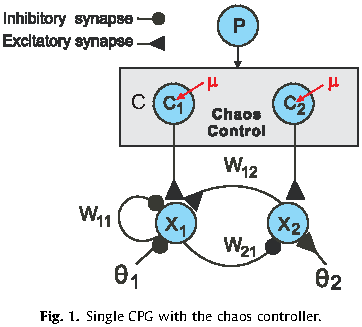
\includegraphics[width=0.6\textwidth]{figs/CPG-overview.pdf}
\end{figure}
\footnote{From [2]}
\end{frame}

\begin{frame}
\frametitle{CPG activity (discrete time dynamics)}
\begin{align*}
\text{\textbf{Neuron state}}&\\
x_i(t+1) &= \sigma\left(\theta_i + \sum\limits^2_{j=1}w_{ij} x_j(t) + c_i^{(p)(t)}\right) \, for~i \in \{1,2\}\\
\text{\textbf{Control signal}}&\\
c_i^{(p)} &= \mu_{(p)}(t)\sum\limits^{2}_{j=1}w_{ij}\Delta_j(t)\\
\Delta_j(t) &= x_j(t) = x_j(t-p)\\
\mu_{(p)} &= \mu_{(p)}(t) + \lambda\frac{\Delta^2_1(t) + \Delta^2_2(t)}{p} \, with~\lambda=0.05
\end{align*}
\footnote{From [1]}
\end{frame}


\begin{frame}
\frametitle{Postprocessing motor neuron signals}
\begin{figure}
\center
\includegraphics[width=1\textwidth]{figs/Postprocessing-signals.pdf}
\end{figure}
\footnote{From [2]}
\end{frame}

\begin{frame}
\frametitle{Different hexapod gaits}
\begin{figure}
\center
\includegraphics[width=1\textwidth]{figs/different-hexapod-gaits.pdf}
\end{figure}
\footnote{From [2]}
\end{frame}

\begin{frame}
\frametitle{Sketched walking patterns}
\begin{figure}
\center
\includegraphics[width=0.8\textwidth]{figs/walking-pattern-sketch.pdf}
\end{figure}
\footnote{From [2]}
\end{frame}

\begin{frame}
\frametitle{Motor pattern learning neuron}
\begin{figure}
\center
\includegraphics[width=0.75\textwidth]{figs/motor-pattern-learning.pdf}
\end{figure}
\footnote{From [2]}
\end{frame}

\begin{frame}
\frametitle{Multi CPG extension}
\begin{figure}
\center
\includegraphics[width=1\textwidth]{figs/multi-CPG-extension.pdf}
\end{figure}
\footnote{From [1]}
\end{frame}

\begin{frame}
\frametitle{Client CPG}
\begin{figure}
\center
\includegraphics[width=0.8\textwidth]{figs/client-CPG.pdf}
\end{figure}
\footnote{From [1]}
\end{frame}

\begin{frame}
\frametitle{Synchronous and asynchronous CPGs}
    \vspace*{-0.4cm}
\begin{figure}
\center
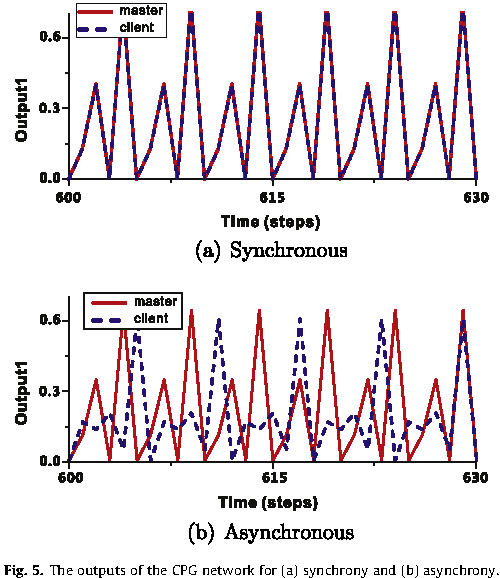
\includegraphics[width=0.55\textwidth]{figs/synchrony-asynchrony.pdf}
\end{figure}
\footnote{From [1]}
\end{frame}

\begin{frame}
\frametitle{Trajectory deviation measure}
\begin{figure}
\center
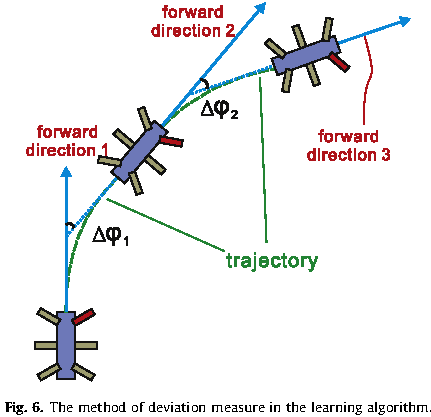
\includegraphics[width=0.8\textwidth]{figs/deviation-measure.pdf}
\end{figure}
\footnote{From [1]}
\end{frame}

\begin{frame}[fragile]
\frametitle{Simulated annealing for leg period learning}
\begin{algorithm}[mathescape]
initialize $C(1)= [1/4 1/24; 4; 4; 4; 4; 4]; \Delta\phi= 0.0; E_1 = 0.0$
repeat:
    At repetition n
    do
        randomly pick a leg l, $l \in [R1; R2; R3; L1; L2; L3]$
        change the period of leg l to a random value, $P(l) \in [4; 5; 6; 8; 9]$
        compare this combination of leg periods, $C'(n)$, to the leg periods of $C(n-1)$
    until $C'(n)$ is a new combination of leg periods
    
    run the robot
    // calculate the evaluation function and its variation
    $E_n = \Delta\phi$
    $\Delta E = E_n - E_{n-1}$
    
    // choose the combination of leg periods
    if $\Delta E < 0$ then
        $C(n) = C'(n)$
    else
        if  $X \geq e^{-\beta \Delta E}$ then // $X \in [0;1], learning~rate~\beta$ 
            $C(n) = C'(n)$
        else
            $C(n) = C(n - 1)$
        end if
    end if
until: The evaluation function $E_n$ is less than a required value $E_{req}$
\end{algorithm}
\end{frame}

\begin{frame}
\frametitle{$\beta$ Tuning (Changing the acceptance rate)}
\begin{figure}
\center
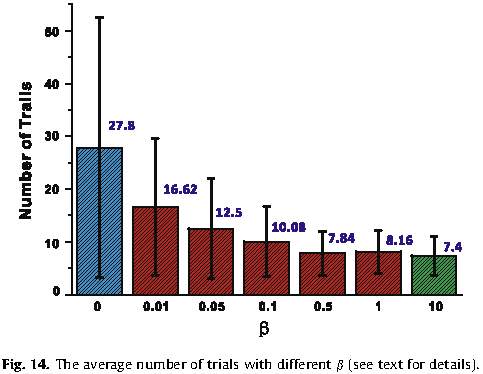
\includegraphics[width=0.7\textwidth]{figs/beta-tuning.pdf}
\end{figure}
\footnote{From [1]}
\end{frame}

\begin{frame}
\frametitle{Learning process}
\begin{figure}
\center
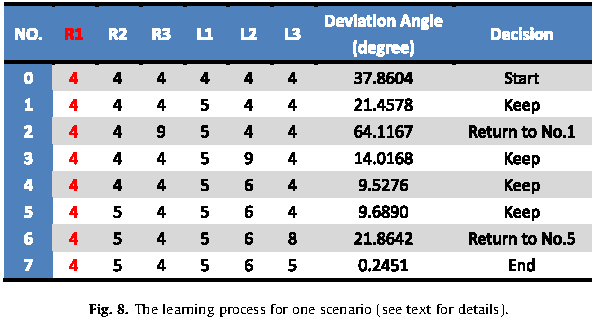
\includegraphics[width=1\textwidth]{figs/learning-process.pdf}
\end{figure}
\footnote{From [1]}
\end{frame}

\begin{frame}
\frametitle{Different leg disabilities}
\vspace*{-0.6cm}
\begin{figure}
\hspace*{-1cm}
\includegraphics[width=0.56\textwidth]{figs/disable-legs-list-1.pdf}
\includegraphics[width=0.56\textwidth]{figs/disable-legs-list-2.pdf}
\end{figure}
\footnote{From [1]}
\end{frame}

\begin{frame}
\frametitle{Leg periods after R1 compensation}
\vspace*{-0.35cm}
\begin{figure}
\hspace*{-1.3cm}
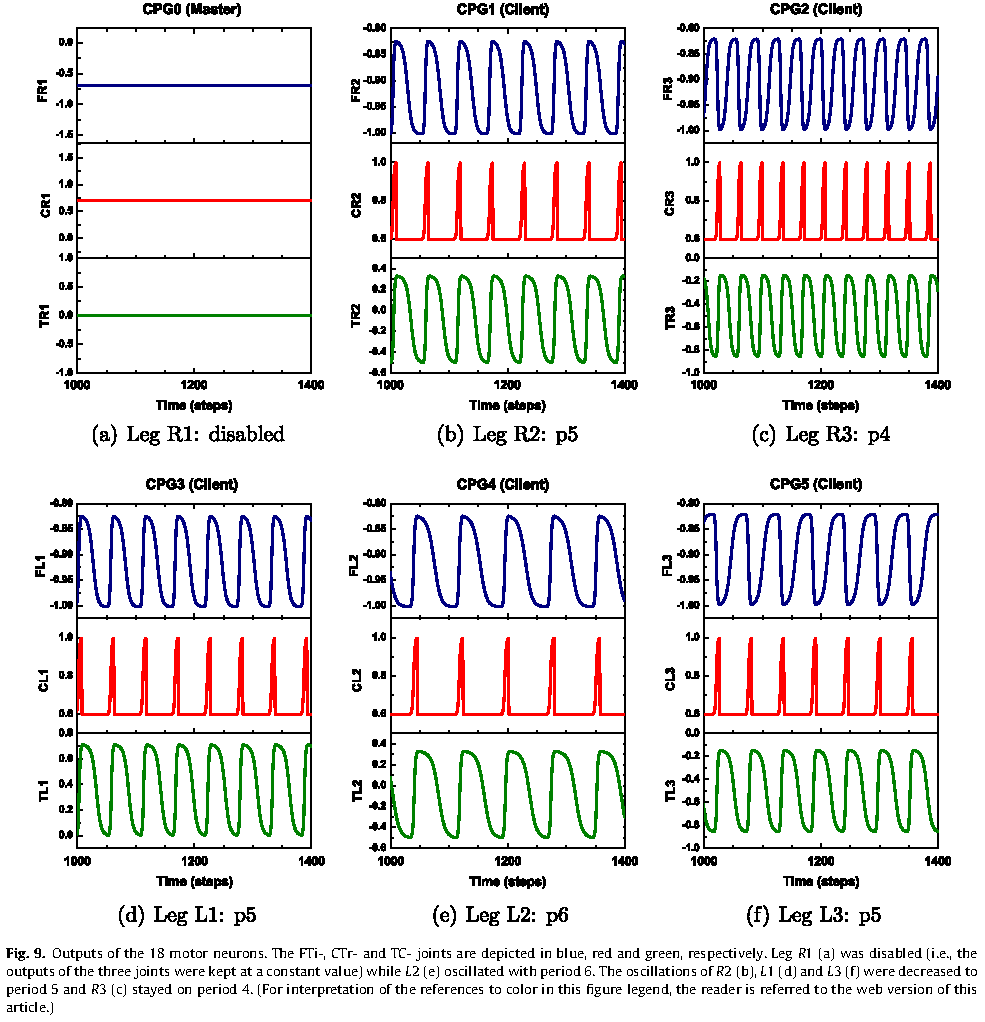
\includegraphics[width=0.8\textwidth]{figs/periods-after-learning.pdf}
\end{figure}
\textbf{\footnote{From [1]}}
\end{frame}

\begin{frame}
    \vspace*{1cm}
    \hspace*{1.1cm}
    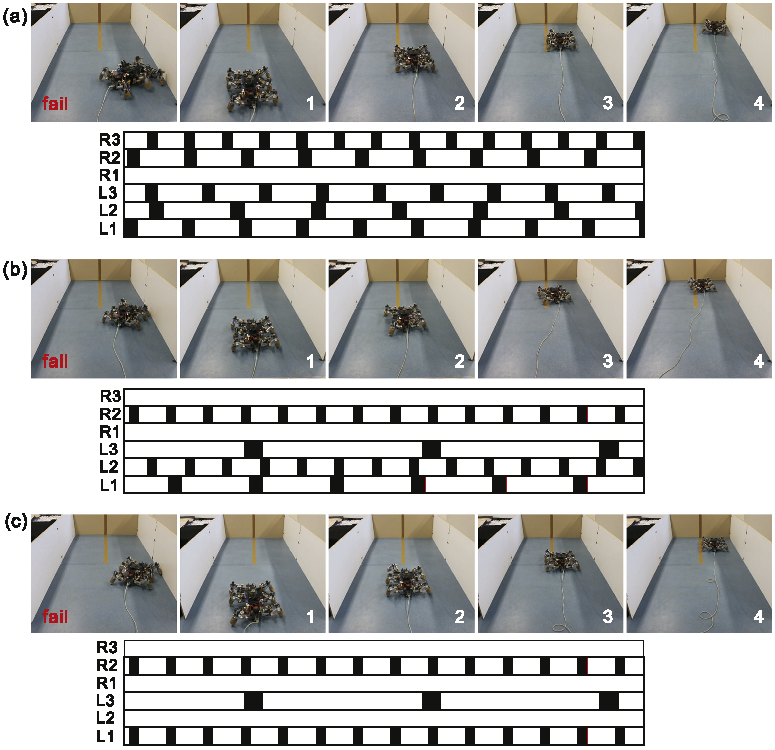
\includegraphics[width=0.8\textwidth]{figs/real-experiments.pdf}
    \footnote{From [1]}
\end{frame}

\begin{frame}
\frametitle{Real performance video}
\begin{figure}
\center
\movie[autostart,showcontrols]{\includegraphics[width=0.6\textwidth]{figs/AMOS.jpg}}{figs/videos/supple_video.wmv}
\end{figure}
\footnote{From [1]}
\end{frame}

\begin{frame}
\frametitle{Comparison to other approaches}
    \hspace*{-0.7cm}
  \centering
  \begin{tabular}{p{2cm}p{4.2cm}p{4.2cm}}
     & \textbf{Ren \& Chen} & \textbf{Cully \& Clune} \\
     \hline
    \textbf{Model} & Chaotic CPG & Gaussian Process \\
    \hline
    \textbf{Additional Prior} & None & Search space \newline premodelling \& \newline  prior performance values\\
    \hline
    \textbf{Optimization} & Simulated Annealing (GD) & Intelligent Trial \& Error \newline (Bayesian Optimization) \\
    \hline
    \textbf{Trials} & Few (1-10) & Few (1-10)
  \end{tabular}
  \\[1cm]
  \textbf{How can the performances be so similar?}
  \footnote{From [1] and [3]}
\end{frame}

\begin{frame}
\frametitle{Keypoints}
\begin{itemize}
\item A chaotic system can be controlled into showing periodic dynamics, so as to be implemented as a CPG to accomplish the locomotion control of a bio-inspired hexapod robot
\item Multiple coupled chaotic CPGs with learning can be used for legged locomotion and malfunction compensation
\item A simulated annealing optimization is sufficient if the basic locomotion mechanism aids the optimization
\item Chaotic ground state can improve the overall performance of a robot and make it easier to search for matching periodicities
\end{itemize}

\end{frame}

\begin{frame}
\frametitle{Flaws}
\begin{itemize}
\item The system does not use any additional sensors to detect malfunction.
\item The PSN/VRN networks and the delay lines make it a beautiful walking machine, but unfortunately make it unable to do anything else.
\item Broken legs are generally not disabled totally, but misbehave in some way (Reduced torque output, incorrect position etc.). This case was not considered. 
\end{itemize}

\end{frame}

\begin{frame}
\newcommand{\quadrat}{(0,0mm)--(0mm,5mm)--(5mm,5mm)--(5mm,0mm)--(0mm,0mm);}
\begin{center}
    \hspace{-8mm}
    \begin{tikzpicture}[overlay]
        {\draw[ETHa,fill=ETHa] \quadrat}\label{ETH1}
    \end{tikzpicture}
    \hspace{10mm}
    \begin{tikzpicture}[overlay]
        {\draw[ETHb,fill=ETHb]\quadrat}\label{ETH2}
    \end{tikzpicture}
    \hspace{10mm}
    \begin{tikzpicture}[overlay]
        {\draw[ETHc,fill=ETHc]\quadrat}\label{ETH3}
    \end{tikzpicture}
    \hspace{10mm}
    \begin{tikzpicture}[overlay]
        {\draw[ETHd,fill=ETHd] \quadrat}\label{ETH4}
    \end{tikzpicture}
    \hspace{10mm}
    \begin{tikzpicture}[overlay]
        {\draw[ETHe,fill=ETHe] \quadrat}\label{ETH5}
    \end{tikzpicture}
    \hspace{10mm}
    \begin{tikzpicture}[overlay]
        {\draw[ETHf,fill=ETHf] \quadrat}\label{ETH6}
    \end{tikzpicture}
    \hspace{10mm}
    \begin{tikzpicture}[overlay]
        {\draw[ETHg,fill=ETHg] \quadrat}\label{ETH7}
    \end{tikzpicture}
    \hspace{10mm}
    \begin{tikzpicture}[overlay]
        {\draw[ETHh,fill=ETHh] \quadrat}\label{ETH8}
    \end{tikzpicture}
    \hspace{10mm}
    \begin{tikzpicture}[overlay]
        {\draw[ETHi,fill=ETHi] \quadrat}\label{ETH9}
    \end{tikzpicture}\\
    \vspace*{1em}
    {\Huge \textbf{Discussion!}}
\end{center}
\vspace*{1.5em}

\begin{itemize}
\item Any questions?
\end{itemize}

\end{frame}


\frame{

  \frametitle{References}
  \begin{itemize}
  \item [\textbf{[1]}] G. Ren, W. Chen. et al., "Multiple chaotic central pattern generators with learning for legged locomotion and malfunction compensation", Information Sciences 294 (2015)
  \item [\textbf{[2]}] S.Steingrube, M. Timme et al., "Self-organized adaptation of a simple neural
circuit enables complex robot behaviour", Nature Physics 6 (2010)
  \item [\textbf{[3]}] A. Cully, J. Clune et al. "Robots that can adapt like animals", Nature 521 (2015)
  \end{itemize}
}
\note{}

\begin{comment}

% Example slides
\begin{frame}
\textbf{Some mathematical specialities}

\ETHbox{0.8\textwidth}{% define the ETHbox
  \begin{theorem}[Murphy (1949)]\label{murphy}
    Anything that can go wrong, will go wrong.
  \end{theorem}
}

\begin{proof}
  A special case of Theorem \ref{murphy} is proven in %\citet{matthews1995}.
\end{proof}
\end{frame}

\begin{titlestyleframe}
\frametitle{Title Page}

\color{white} The title page is created using the \texttt{\textbackslash titleframe} command.

The title page background can also be used on other frames (or for a customised title frame) using the \texttt{titlestyleframe} environment.
\end{titlestyleframe}

\begin{frame}
\frametitle{Normal Frame}
The normal frame looks like this. It is created using the \texttt{frame} environment.
\end{frame}
\begin{inverseframe}
  \frametitle{Inverse Slides}
  %\color{white}
The inverted frame looks like this. It is created using the \texttt{inverseframe} environment.

 
\end{inverseframe}

\begin{minimalframe}
  \frametitle{Minimal Frame}
The minimal frame looks like this. It is created using the \texttt{minimalframe} environment.
  
\end{minimalframe}

\begin{minimalframe} 
\end{minimalframe}

\end{comment}

\end{document}
